
\section{Scheduling statico}
Lo scheduling statico di una pipeline è una tecnica di ottimizzazione usata nei processori con pipelining (soprattutto nelle architetture RISC e VLIW) per ridurre o eliminare i hazard (conflitti di dati, di controllo o strutturali) senza dover ricorrere a meccanismi di risoluzione hardware dinamici. Statico significa che lo scheduling viene fatto dal compilatore, in fase di compilazione, non dal processore a runtime. L'idea è che il compilatore riordini le istruzioni in modo da minimizzare i cicli di stallo (stall) e sfruttare al massimo la pipeline.

\section{Scheduling dinamico}
Con scheduling dinamico intendiamo tecniche hardware che \textit{on the fly}, durante l'esecuzione, cambiano l'ordine di processo di determinate operazioni per risolvere i conflitti ed evitare quando possibile lo stallo della pipeline. I vantaggi di uno scheduling dinamico sono molteplici:

\begin{itemize}
    \item Permette a codice compilato per una determinata architettura di essere efficiente anche su un'architettura diversa, eliminando parzialmente la relazione che sussite tra efficienza e compilazione;
    \item Permette di gestire casi in cui alcune dipendenze non sono note a tempo di compilazione (riferimenti in memoria e salti dipendenti dai dati);
    \item Permette al processore di tollerare dei ritardi non prevedibili a tempo di compilazione (cache miss).
\end{itemize}

Il datapath di una pipeline deve essere gestito da un'opportuna unità di controllo, che risolva potenziali condizioni di \textit{hazard}. Questa unità è responsabile di rilevare il problema e risolverlo bloccando la pipeline a partire da un certo stadio in poi, inserendo delle \textit{bolle}. Per rendere possibile questo controllo è necessario propagare dalla fase ID in poi gli indici deglio operandi, in modo tale che l'unità di controllo possa rilevare possibili conflitti. 

\subsection{Forward paths}
Il vincolo sulla dipendenza RAW riguarda \textit{vere dipendenze}, ovvero dipendenze dettate dal problema produttore-consumatore tra le istruzioni, e sono indipendenti dall'architettura (riguardano in senso logico il flusso di esecuzione del codice). Inserire un path diretto [output ALU $\rightarrow$ registro operandi] permette di rilassare il vincolo di dipendenza e fare in modo che l'unità di controllo possa risolvere il potenziale conflitto.  
In altre parole, si cambia il \textit{grafo delle dipendenze} tra le operazioni.

\begin{figure}[ht]
    \centering
    \setlength{\fboxrule}{0.5pt} % spessore sottile
    \setlength{\fboxsep}{0pt}    % senza spazio interno
    \fbox{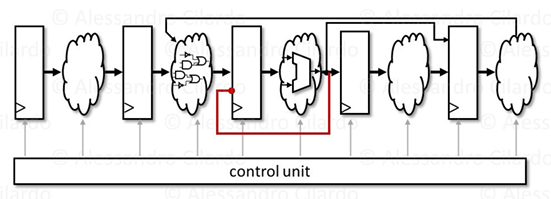
\includegraphics[width=0.6\textwidth]{fig/chapter_2/basic_forwarding.png}}
\end{figure}

\begin{info}
    Grafo delle dipendenze: grafo orientato in cui le istruzioni costituiscono i nodi, gli archi invece rappresentano le dipendenze tra queste.
\end{info}

Il costo di questi benefici è una notevole complicazione dell'hardware. Osserviamo inoltre che lo scheduling dinamico è utlizzabile insieme allo scheduling statico effettuato dal compilatore: una tecnica non prescinde l'altra. \\ \noindent
Osserviamo che in uno schema pipeline a cinque stages di base, dove non contempliamo istruzioni fuori ordine, è verificata sempre la condizione: \textit{una micro-operazione di un'istruzione precedente è sempre eseguita prima della stessa o una successiva micro-operazione di un'istruzione successiva}. In altre parole, se un'istruzione A precede un'istruzione B, l'operazione di \textit{lettura operandi} dell'istruzione A è eseguita prima delle operazioni EX, MEM e WB dell'istruzione B. Di conseguenza, in questo schema semplificato non sono possibili hazards di tipo WAW e WAR. 
Questo è in generale \textbf{falso} per gli approcci basati sul rescheduling delle operazioni. 

\subsection{Esecuzione out-of-order}
Un'unità funzionale, come un moltiplicatore o un divisore, può essere internamente organizzata come una pipeline. In questo modo l'unità può iniziare una nuova operazione ad ogni ciclo, pur impiegando diversi cicli per completare un'operazione. 

\begin{info}
    L'\textbf{initialization interval} (II) è il numero di cicli di clock che devono passare prima di poter avviare una nuova iterazione della pipeline. Questo limite è imposto dall'hardware.
\end{info}

Se l'II dell'unità funzionale serializzata è minore della latenza totale dell'unità, allora più micro-operazioni possono coesistere nella stessa unità funzionale, pur attraversandola sempre in ordine. Se lo stage EXE contiene più di un'unità funzionale specializzata, ognuna con diverse latenze, è necessario introdurre l'esecuzione \textit{out of order}. 
Complicando in questo modo l'hardware, è necessario fare delle considerazioni: differenti unità funzionali possono completare l'esecuzione nello stesso ciclo $\rightarrow$ hazard strutturali sull'insieme dei registri $\rightarrow$ WAW hazard; se l'hardware supporta molteplici operazioni di lettura operandi concorrenti, sono possibili hazards strutturali sullo stage EXE (?); Sono possibili hazard di tipo WAR, e gli hazards ti tipo RAW sono più frequenti. 
Nelle architetture superscalari il processore può emettere ed eseguire più istruzioni nello stesso ciclo di clock. Questo implica che diverse unità funzionali possano aver bisogno, contemporaneamente, di leggere o scrivere registri. Per esempio, due istruzioni aritmetiche emesse nello stesso ciclo possono richiedere entrambe di leggere due operandi e di scrivere un risultato; se il file dei registri fosse accessibile da una sola porta di lettura e scrittura, ci sarebbe un collo di bottiglia che impedirebbe l'esecuzione parallela. Per questo motivo i registri devono essere multiportati, cioè progettati per permettere più accessi simultanei da locazioni diverse, in modo da garantire che le varie istruzioni in issue nello stesso ciclo possano ottenere i loro operandi o aggiornare i risultati senza conflitti. Rendere i registri multiporting è difficile principalmente per ragioni di complessità circuitale e di costo. Ogni porta aggiuntiva di lettura o scrittura richiede linee di accesso dedicate, logica di decodifica separata e soprattutto un incremento del numero di connessioni interne, il che fa crescere in modo quasi quadratico l'area del circuito e la capacità parassita. Questo significa che più porte si aggiungono, più aumenta il consumo energetico e più rallenta il tempo di accesso ai registri.
\\ \noindent Avere a che fare con molteplici scritture implica scegliere una strategia di rilevazione della dipendenza e di risoluzione: se si sceglie di rilevare il conflitto già in fase di ID, il processore deve subito confrontare i registri di destinazione delle istruzioni decodificate con quelli delle istruzioni più vecchie ancora in pipeline. Per non perdere l'informazione man mano che le istruzioni avanzano, si usa una catena di shift registers che traccia la distanza (in termini di stadi di pipeline) fino a quando l'istruzione precedente eseguirà il WB. In questo modo, fin dall'inizio si sa che una certa istruzione dovrà aspettare un certo numero di cicli prima di poter scrivere in sicurezza. Il vantaggio è che i conflitti sono gestiti in anticipo, evitando bolle tardive. Lo svantaggio è che servono comparatori e logica aggiuntiva in ID, e gli shift register complicano l'hardware.
L'alternativa è rilevare il conflitto il più tardi possibile, cioè attendere che le istruzioni arrivino in prossimità della fase di write-back e solo lì controllare se due istruzioni stanno tentando di scrivere lo stesso registro nello stesso ciclo. Questo riduce la complessità logica in ID e alleggerisce la pipeline nei primi stadi, ma aumenta la probabilità di dover bloccare o annullare (stall o flush) istruzioni già avanzate nella pipeline. In altre parole: hardware più semplice, ma più penalità in caso di conflitti.
In generale conviene rilevare i conflitti presto (in ID con shift register) quando si ha un'architettura aggressivamente superscalare o molto profonda, dove i conflitti diventano frequenti e lo stall tardivo sarebbe molto costoso.
Gli hazard possono essere significativamente ridotti introducendo \textbf{isolated type registers}. Ciò significa che, invece di avere un unico file di registri condiviso da tutte le unità funzionali, il processore suddivide i registri in più gruppi separati, ciascuno dedicato a un certo “tipo” di istruzione o unità. Per esempio, ci possono essere registri isolati per le operazioni intere, altri per le operazioni in virgola mobile etc. La separazione riduce drasticamente le probabilità di conflitto, perché istruzioni appartenenti a domini funzionali diversi non competono per lo stesso insieme di registri. Inoltre, avere registri specializzati permette anche di ridurre la complessità del multiporting, dato che ogni file di registri isolato può essere più piccolo e più facile da gestire in parallelo.
\\
L'idea chiave è separare la fase ID in due fasi indipendenti, \textbf{instruction issue} e \textbf{operand read}. L'instrucion issue consiste nell'\textit{accettare} l'istruzione, riservando risorse per tracciarla in stages successivi, e ciò viene di solito performato \textit{in ordine}; l'operand read invece aspetta che gli operando siano pronti, ed è tipicamente performate \textit{out of order}.

\begin{figure}[ht]
    \centering
    \setlength{\fboxrule}{0.5pt} % spessore sottile
    \setlength{\fboxsep}{0pt}    % senza spazio interno
    \fbox{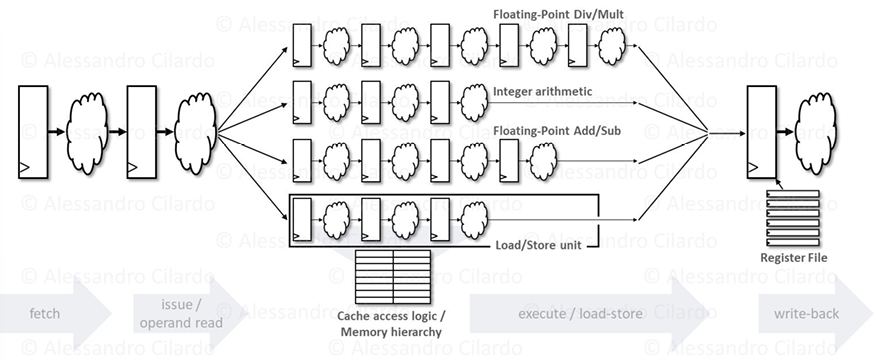
\includegraphics[width=0.6\textwidth]{fig/chapter_2/out_of_order.png}}
\end{figure}

Nella trattazione teorica qui presentata conviene trattare l'unità di load/store (MEM) come un'unità funzionale al pari delle unità funzionali dedite alle operazioni aritmetico-logiche. 

\subsection{Scoreboard}
In questa tecnica di implementazione dell'unità di controllo facciamo delle assunzioni: 
\begin{itemize}
    \item L'issue di un'istruzione ovviene in ordine, e in questa fase vengono rilevati hazards strutturali e WAW;
    \item L'operand read avviene, così come la fase EX e la fase di completamento, out-of-order. Inoltre le dipendenze sui dati sono risolte dinamicamente;
    \item Non vi sono espliciti forwarding paths;
    \item Per ora ci disinteressiamo del modello delle eccezioni/interruzioni.
\end{itemize}

La logica per le fasi issue e operand read sono gestite attraverso due tabelle (\textbf{unit status table} e \textbf{register status table}) dall'unità di controllo.

\begin{figure}[ht]
    \centering
    \setlength{\fboxrule}{0.5pt} % spessore sottile
    \setlength{\fboxsep}{0pt}    % senza spazio interno
    \fbox{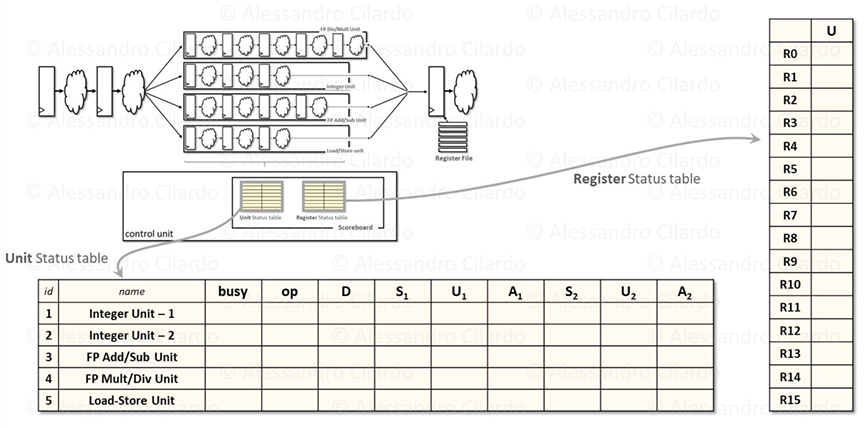
\includegraphics[width=0.6\textwidth]{fig/chapter_2/scoreboard.png}}
\end{figure}

\noindent La unit table ha tante righe quante le unità funzionali e i seguenti campi:

\begin{description}[style=nextline,leftmargin=3.45cm,labelwidth=2.8cm,labelsep=0.4cm,font=\ttfamily\bfseries, itemsep=0.01em]
\item[id] Intero che identifica l'unità funzionale
\item[name] Nome dell'unità funzionale
\item[busy] Flag che indica se l'unità è occupata
\item[op] Specifica operazione righiesta all'unità funzionale 
\item[D] Indice del registro destinazione 
\item[$S_i$] Indice dell'i-esimo registro sorgente    
\item[$U_i$] Id dell'unità che eventualmente sta processando il valore che sarà scritto in $S_i$ (=0 se è già disponibile)
\item[$A_i$] Flag che verifica se il valore nel registro è già disponibile per la lettura  
\end{description}

\noindent Per quanto riguarda la Register Status Table, questa ha tante riche quanti sono i registri e l'unico campo U $\rightarrow$, che contiene l'id dell'unità che evnentualmente sta processando il valore che verrà scritto nel registro (=0 se già disponibile).
\\ \noindent Le istruzioni sono recuperate dalla pipeline in ordine e poi possono trovarsi in una delle seguenti fasi: Issue, Operand Read, Execute o Write Back. 
Le regole per aggiornare le tabelle sono queste:

\begin{itemize}
    \item Un'istruzione viene \textit{accettata} (issued) solo se:
    \begin{itemize}
        \item L'unità funzionale richiesta è libera (busy = 0);
        \item Il registro di destinazione non è già segnato (U=0 nella register status table);
    \end{itemize}
    \item L'Operand Read è performata solo quando entrambi i registri sorgente sono disponibili;
    \item Quando viene performata Operand Read, i flag $A_1$ e $A_2$ vengono resettati;
    \item L'esecuzione procede secondo la pipeline dell'unità funzionale; 
    \item Il WriteBack avviene solo se non ci sono Operand Read sospese su tutte le unità funzionali che aspettano il registro che si sta cercando di scrivere; Una volta effettuato il WB, le entry della tabella relative all'istruzione completata vengono liberate.
\end{itemize}

\noindent Una vola che un'istruzione viene accettata, le tabelle di scoreboard vengono aggiornate per tenere traccia delle unità e dei regeistri coinvolti. Formalmente:

\begin{figure}[ht]
    \centering
    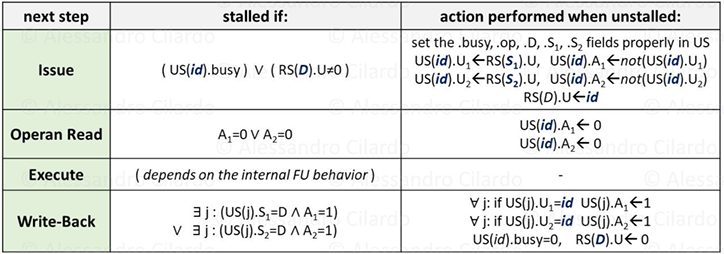
\includegraphics[width=0.8\textwidth]{fig/chapter_2/transition_rules.png}
\end{figure}

\noindent Si consultino le slides del corso per un esempio sulla tecnica dello scoreboard. In sintesi, questa tecnica di gestione previene gli hazards in questo modo: i RAW sono risolti tenendo traccia delle dipendenze tra le istruzioni che sono già state accettate; i WAR sono risolti ritardando il WB finchè i registri scrivendi non vengono letti, e ritardando la lettura dei registri alla fase Read Operands; i WAW sono risolti a monte ritardando l'issue di un'istruzione finchè l'istruzione precedente non completa la scrittura del registro destinazione. Con questa soluzione, comunque l'IPC massimo resta sempre 1. Osserviamo che i dati sono gestiti da registri dell'architettura, e questa è una limitazione chiave che vorremmo superare, poichè è causa di molti hazards di tipo WAR e WAW. 

\begin{warn}
    Gli hazards RAW sono causati da dipendenze intrinseche delle istruzioni. Gli hazards WAR e WAW sono causate da dettagli implementativi (i registri), e pongono solo dei vincoli sullo scheduling.
\end{warn}

\noindent Il limite principale di questa tecnologia è sicuramente il fatto che la gestione avviene attraverso i registri. Le false dipendenze sono causate proprio dalla numero limitato di registri. Ciò non è tanto dovuto ai limiti fisici legati allo spazio sul silicio su cui realizzarli, quanto più è legato ai bit riservati nella codifica di un istruzione per specificare un determinato registro sorgente/destinazione. 
Questo limite emerge soprattutto con i loop (consultare le slides del corso per il chiaro esempio in cui emerge il calo di performance pur assumendo la perfetta predizione del salto). 

\section{L'algoritmo di Tomasulo}
Si tratta di un algoritmo inventato dall'informatico di IBM Robert Tomasulo, passato alla storia per aver \textit{inventato} l'algoritmo che ha permesso l'esistenza dei processori che eseguissero istruzioni non in ordine. 
Gli ingredienti chiave dell'algoritmo sono le \textbf{reservation stations}: Le reservation stations sono dei buffer associati alle unità funzionali di un processore out-of-order. Servono a tenere in sospeso le istruzioni in attesa che i loro operandi diventino disponibili. In pratica, quando un'istruzione viene decodificata non entra subito nell'unità funzionale: viene invece “prenotato” uno slot in una reservation station, che contiene il tipo di operazione da eseguire, i riferimenti agli operandi (o i loro valori, se già disponibili) e il registro destinazione. Così, più istruzioni possono essere emesse in parallelo senza bloccare la pipeline, anche se non hanno ancora tutto ciò che serve per l'esecuzione.
\\ \noindent L'idea di base dell'algoritmo è schedulare dinamicamente istruzioni in modo che possano iniziare appena gli operandi diventano disponibili, e duplicare i valori degli operandi (ovvero rinominare i registri) per evitare inutili hazards. Un altro elemento chiave è il Common Data Bus (CDB): quando un'unità funzionale calcola un risultato, lo invia sul bus comune, e tutte le reservation stations che aspettavano quel valore possono aggiornarlo immediatamente. In particolare, il CDB comunica la coppia (id, value) dove id è l'identificativo dello slot della RS a cui è stato assegnato il valore. 

\begin{figure}[ht]
    \centering
    \setlength{\fboxrule}{0.7pt} % spessore sottile
    \setlength{\fboxsep}{0pt}    % senza spazio interno
    \fbox{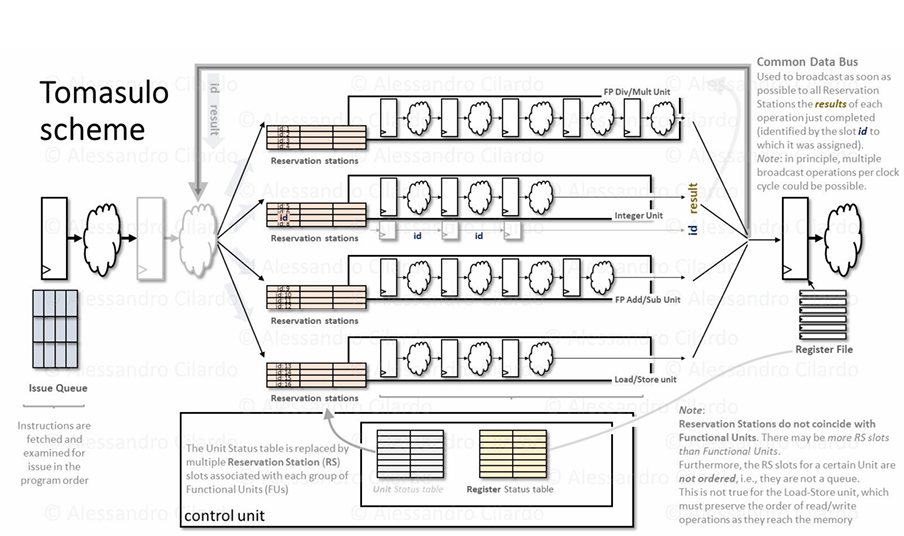
\includegraphics[width=0.8\textwidth]{fig/chapter_2/tomasulo_scheme.png}}
\end{figure}

Rispetto allo scoreboard, le Unit Status tables vengono rimpiazzate dalle Tomasulo Tables (Reservation Stations RS), che in generale possono essere più delle unità funzionali. Queste tabelle vengono assegnate in rapporto n:1 ad un'unità funzionale, e sono divise in slot, uno per ogni riga della singola tabella. I campi della tabella sono:

\begin{description}[style=nextline,leftmargin=3.45cm,labelwidth=2.8cm,labelsep=0.4cm,font=\ttfamily\bfseries, itemsep=0.01em]
\item[id] Intero che identifica univocamente lo slot
\item[name] Nome dell'unità funzionale + slot number
\item[busy] Flag che indica se l'unità funzionale è occupata
\item[op] Specifica operazione righiesta all'unità funzionale 
\item[$st_i$] Indice dello slot della RS che fornirà eventualmente il valore dell'i-esimo operando (=0 se il dato è già disponibile e può essere direttamente \textbf{copiato} dai registri) 
\item[$V_i$] Valore dell'i-esimo operando, \textbf{copiato} 
\item[$Ad$] Usato per mantenere l'eventuale offset in caso di indirizzamento base+offset e poi l'indirizzo effettivo (solo nelle operazioni di load/store).  
\end{description}


\begin{figure}[ht]
    \centering
    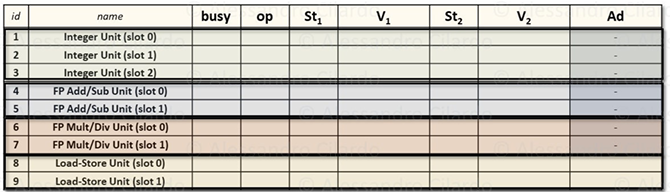
\includegraphics[width=0.6\textwidth]{fig/chapter_2/tomasulo_tables.png}
\end{figure}

\noindent La register status table invece contiene i campi nome registro e St, ovvero l'indice dello slot della reservation station che fornirà il valore (=0 se già disponibile). 
Occorre fare un'osservazione sull'unità di load/store (LSU): La RS associata (chiamata anche Load/Store buffer) mantiene anche i dati da archiviare e l'indirizzo di memoria target. In un primo momento, in caso di indirizzamento base+offset, nel campo aggiuntivo verrà conservato l'offset, e in un secondo momento verrà conservato l'indirizzo effettivo. Osserviamo inoltre che la LSU garantisce l'ordinamento degli accessi in memoria. Questo è cruciale per sequenze di operazioni verso lo stesso indirizzo che includono almeno una Store. La LSU garantisce che le operazioni di lettura/scrittura allo stesso indirizzo accedano in memoria in ordine. Possono essere implementati all'interno della stessa tabella dei \textit{forward paths} nel campo valore, dove nel caso di letture che seguono una scrittura il valore può essere direttamente passato, comparando il campo \textit{effective address}.
\\ \noindent Vediamo nel dettaglio come funziona lo schema di Tomasulo:

\begin{itemize}
    \item Le istruzioni sono recuperate in ordine, poi seguono i passi Issue, Execute, Write Back;
    \item Un'istruzione viene accettata se un appropriato slot è disponibile nella RS (anche se le unità funzionali sono occupate);
    \item Una volta accettata, se possibile vengono copiati i dati necessari, oppure si rtiene traccia delle \textbf{operazioni} sospese che forniranno il dato più tardi;
    \item L'esecuzione avviene quando tutti i dati sono disponibili e copiati nei campi $V_i$ edlla RS;
    \item Il WB avviene quando il CDB è disponibile, in modo che il risultato può essere trasmesso in broadcast con l'id dello slot che ha generato quel risultato. In questo modo, tutte gli slot in attesa del risultato da quell' ID possano ricevere contemporaneamente il valore. 
\end{itemize}

\noindent Notiamo subito che gli hazards strutturali sono ancora possibili nel caso che le tabelle vadano in overflow. Ma costruire RS più capienti è meno costoso di aggiungere unità funzionali. 

\begin{figure}[ht]
    \centering
    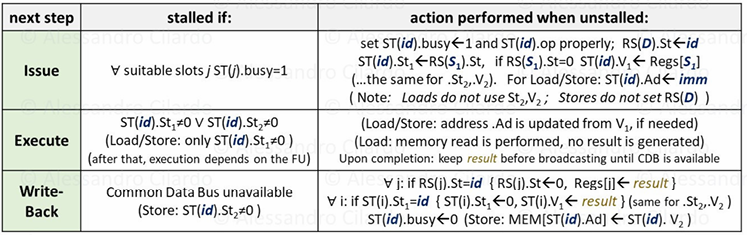
\includegraphics[width=0.8\textwidth]{fig/chapter_2/tomasulo_transitions.png}
\end{figure}

\noindent Il miglioramento di performance, una volta evitati i conflitti dovuti alle false dipendenze, è palese ed è visibile nell'esempio presentato nelle slides del corso. 

\begin{figure}[ht]
    \centering
    \setlength{\fboxrule}{0.7pt} % spessore sottile
    \setlength{\fboxsep}{0pt}    % senza spazio interno
    \fbox{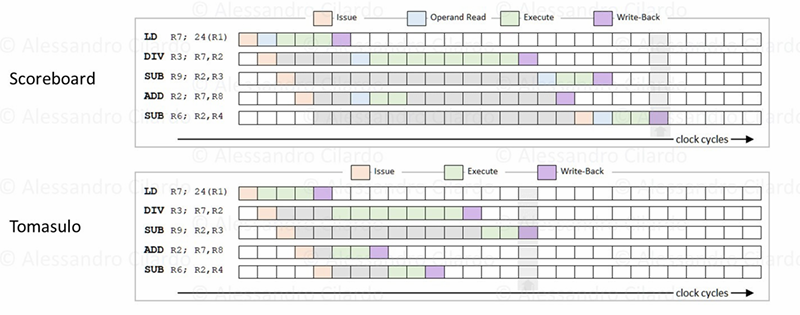
\includegraphics[width=0.8\textwidth]{fig/chapter_2/scoreboard_vs_tomasulo.png}}
\end{figure}

\noindent Il miglioramento è ravvisabile soprattutto nei loop ristretti, dove vengono usati in rapida successione gli stessi registri. Qui è lampante la potenza del \textit{renaming} dei registri. 

\begin{info}
    Un'interessante considerazione riguarda il \textit{software loop unrolling}, ovvero una naturale ottimizzazione a livello software della pipeline e dello scheduling dinamico. Di fatto si \textit{srotola} parzialmente il loop, in modo da rendere i branch meno frequenti ed utilizzare più registri in maniera esplicita. Questa operazione viene fatta dal programmatore o dal compilatore. Questa scelta potrebbe causare la crescita del codice, e di conseguenza potrebbero verificarsi più cache miss in fase di IF (riduzione della località spaziale), e per codici particoralmente complessi potrebbe risultare oneroso rilevare parallelismo, analizzare le dipendenza riguardanti la memoria e risistemare le condizioni di fine loop.
\end{info}
